%! suppress = FileNotFound
\documentclass{article}
%TODO UPDATE CALCULATIONS WITH SIGNIFICANT FIGURES
\usepackage[utf8]{inputenc}
\usepackage[letterpaper, portrait, margin=1in]{geometry}
\usepackage{graphicx} % Required for inserting images
\usepackage{amsmath}
\usepackage{float}

%TODO ONCE I GET THE EXACT VALUES OF THINGS I NEED TO UPDATE THE VALUES IN THE DOCUMNT AND REDO SOM OF THE CALCULATIONS

\usepackage{indentfirst}
\usepackage{hyperref}
%\usepackage{longtable}
%\usepackage{multicol}
%\usepackage{xtab}
%\usepackage{table*}
%\usepackage{tabularx}
\graphicspath{{./latex\_figures/}}
%\usepackage{supertabular}

\title{Spring Potential Energy Lab}
\author{Aiden Ma}
\date{October 17th, 2023}

\begin{document}
    \maketitle
    
    \newpage
    
    %table of contents
    \tableofcontents
    
    \newpage
    
    
    \section{Introduction}\label{sec:introduction}
        In this lab, we will be investigating the rate of change of mechanical energy over time of an oscillating mass on a spring.
        We will measure the spring constant of the spring, as well as the position and velocity of the mass oscillating vertically on a spring.
    
    
    \section{Relevant Knowledge and Definitions}\label{sec:relevant-knowledge-and-definitions}
        \begin{itemize}
            \item \textbf{Mechanical energy} is the sum of kinetic energy and potential energy.
            The unit for all forms of energy is the joule (J).
            \item \textbf{Kinetic energy} is the energy of motion.
            The equation for kinetic energy is $K = \frac{1}{2}mv^2$, where $m$ is the mass of the object and $v$ is the velocity of the object.
            \item On the other hand, \textbf{potential energy} is the energy of position relative to others.
            Potential energy is stored energy that can be converted into kinetic energy.
            Potential energy comprises a large series of different forms of energy, two of which are important for this lab.
            \begin{itemize}
                \item \textbf{Spring potential energy} is the energy stored in a spring when it is stretched or compressed.
                The equation for spring potential energy is $U = \frac{1}{2}k(\Delta x)^2$, where $k$ is the spring constant and $\Delta x$ is the distance the spring is stretched.
                \item \textbf{Gravitational potential energy} is the energy stored in an object due to its position another position.
                The equation for gravitational potential energy is $U = mgh$, where $m$ is the mass of the object, $g$ is the acceleration due to gravity, and $h$ is the height of the object another position.
            \end{itemize}
            \item The \textbf{spring} constant is the amount of force required to stretch the spring 1 meter.
            The unit for spring constant is newtons per meter ($\frac{\text{N}}{\text{m}}$).
            \item A \textbf{cycle} is one complete oscillation of the spring from peak to peak.
            \item A \textbf{peak} is the highest point of the oscillation.
        \end{itemize}

    \section{Goal}\label{sec:goal}
        To determine the rate of change of mechanical energy with respect to time of a mass oscillating vertically by the use of a spring.
    
    \section{Materials}\label{sec:materials}
        \begin{itemize}
            \item Laptop with Logger Pro
            \item Spring
            \item 3x 20g masses
            \item 1x 50g mass
            \item Ultrasonic motion detector
            \item Length measuring apparatus
            \item Mass holder
            \item Test tube stand %TODO (what is this called?)
            \item Test tube clamp
        \end{itemize}
    
    
    \section{Procedure}
        \noindent Measuring the spring constant:
        \begin{enumerate}
            \item Set up the measuring apparatus so that the spring is hanging vertically from the length measuring apparatus with no mass attached except for the mass holder.
            \item Set the length measuring apparatus to zero at the current spring length.
            \item Add the 20g mass to the spring and record the length of the spring.
            \item Repeat step 3 until you have added all 3 20g masses.
            \item Remove all the masses and add the 50g mass to the spring and record the length of the spring.
            \item Add a 20g mass to the spring and record the length of the spring.
        \end{enumerate}
        
        \noindent Measuring the change in mechanical energy over time:
        \begin{enumerate}
            \item Set up the measuring apparatus so that the spring is hanging vertically from the ultrasonic motion detector.
            \item Open logger pro and set up the motion detector.
            \item Set up the spring so that it is at its equilibrium position.
            \item Record the position of the spring.
            \item Add a 50g mass to the spring, let the mass rest in its equilibrium position while not oscillating, and record the position of the spring.
            \item Pull the mass down 5cm and release it.
            \item Record the position of the spring every 0.05 seconds using the ultrasonic motion detector for 415 seconds.
        \end{enumerate}
    
    
    \section{Data}
        
        \subsection{Spring constant}\label{subsec:spring-constant-data}
            \begin{table}[H]
                \centering
                \begin{tabular}{|c|c|}
                    \hline
                    Mass ($m$) [kg]                & Length ($\Delta x$) [cm] \\
                    \hline
                    $m_0$                          & 0.00                     \\
                    \hline
                    $m_0 + 0.02$ (1x 20g)          & 1.95                     \\
                    \hline
                    $m_0 + 0.04$ (2x 20g)          & 3.90                     \\
                    \hline
                    $m_0 + 0.05$ (1x 50g)          & 4.90                     \\
                    \hline
                    $m_0 + 0.06$ (3x 20g)          & 5.85                     \\
                    \hline
                    $m_0 + 0.07$ (1x 20g + 1x 50g) & 6.85                     \\
                    \hline
                \end{tabular}
                \caption{Spring extention data}\label{tab:spring-extention-data}
            \end{table}
        
        \subsection{Length of $x_0$ and $x$ for a 50 gram mass}
            Experimentally the distance of $x_0$ above the motion detector was 32.8 cm. %todo update this value with a more accurate value
            
            Experimentally the distance of $x$ above the motion detector was 24.0 cm. %todo update this value with a more accurate value
        
        \subsection{Change in mechanical energy over time}\label{subsec:change-in-mechanical-energy-over-time-data}
            %todo add a table of data
    
    
    \section{Analysis}\label{sec:analysis}
        
        \subsection{Calculating the spring constant}\label{subsec:calculating-the-spring-constant}
            %TODO add a graph showing linear fit of the spring constant data
            
            Free body diagram of the mass holder and the added masses:
            %figure FBD
            \begin{figure}[H]
                \centering
                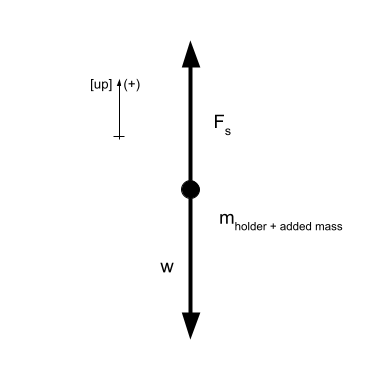
\includegraphics[width=0.3\linewidth]{FBD}
                \caption{Free body diagram of the mass holder and the added mass}
                \label{fig:FBD}
            \end{figure}
            
            Since the mass is at rest before and after adding the masses, $F_{net}^{\text{original}} = 0$, $F_{net}^{\text{new}} = 0$.
            Since the only force acting on the mass is gravity and the spring force, and the mass is at rest, the spring force must be equal to the force of gravity.
            Therefore, we can use the following formula to calculate the spring constant:
            
            %TODO FIX THESE EQUATIONS
            
            \begin{equation}
                \begin{aligned}
                    F_{\text{net}}^{\text{new}} &= 0 \\
                    F_{\text{spring}}^{\text{new}} - F_{\text{gravity}}^{\text{new}} &= 0 \\
                \end{aligned}\label{eq:spring constant equation_pt1}
            \end{equation}
            
            Since $F_{net}^{\text{original}} = 0$:
            \begin{equation}
                \begin{aligned}
                    \notag
                    F_{\text{net}}^{\text{original}} &= 0 \\
                    F_{\text{spring}}^{\text{original}} - F_{\text{gravity}}^{\text{original}} &= 0 \\
                \end{aligned}\label{eq:spring constant equation_pt2}
            \end{equation}
            
            Plugging back into equation~\ref{eq:spring constant equation_pt1}:
            
            \begin{equation}
                \begin{aligned}
                    \notag
                    F_{\text{spring}}^{\text{new}} - F_{\text{gravity}}^{\text{new}} &= 0 \\
                    F_{\text{spring}}^{\text{new}} - F_{\text{gravity}}^{\text{new}} &= F_{\text{spring}}^{\text{original}} - F_{\text{gravity}}^{\text{original}} \\
                    F_{\text{spring}}^{\text{new}} + F_{\text{spring}}^{\text{original}}- F_{\text{gravity}}^{\text{new}} - F_{\text{spring}}^{\text{original}} &= 0 \\
                    \Delta F_{\text{spring}} - \Delta F_{\text{gravity}} &= 0 \\
                \end{aligned}\label{eq:spring constant equation_pt3}
            \end{equation}
            
            Thus, we can solve for $k$ as follows:
            \begin{equation}
                \begin{aligned}
                    \Delta F_{\text{spring}} - \Delta F_{\text{gravity}} &= 0 \\
                    \Delta F_{\text{spring}} &= \Delta F_{\text{gravity}} \\
                    k\Delta x &= g \Delta m \\
                    k &= \frac{g \Delta m}{\Delta x} \\
                \end{aligned}\label{eq:spring constant equation}
            \end{equation} \\
            %todo move tag to the end of the equation list
            
            In this case, $\Delta m$ is the mass of the mass added to the spring, and $\Delta x$ is the change in length of the spring when that mass is added.
            
            Using equation~\ref{eq:spring constant equation}, we can calculate the spring constant for each mass added to the spring.
            For example, if we take the data from the first mass, we can calculate the spring constant as follows:
            
            \begin{equation}
                \begin{aligned}
                    \notag
                    k &= \frac{g \Delta m}{\Delta x} \\
                    k &= \frac{(9.8 \frac{\text{ m}}{\text{ s}^2})(0.02 \text{ kg})}{0.0195 \text{ m}} \\
                    k &= 10.05 \frac{\text{ N}}{\text{ m}} \\
                \end{aligned}\label{eq:example spring constant equation}
            \end{equation}
            %with uncertainty calculations
            % delta x has an uncertainty of 0.0005 m
            
            
            %TODO do uncertainty calculations later
            \begin{table}[H]
                \centering
                \begin{tabular}{|c|c|c|}
                    \hline
                    Added Mass ($m$) [kg] & Length ($\Delta x$) [m] & Spring Constant ($k$) [$\frac{\text{N}}{\text{m}}$] \\
                    \hline
                    0.02                  & 0.0195                  & 10.05                                               \\
                    \hline
                    0.04                  & 0.0390                  & 10.05                                               \\
                    \hline
                    0.05                  & 0.0490                  & 10.00                                               \\
                    \hline
                    0.06                  & 0.0585                  & 10.05                                               \\
                    \hline
                    0.07                  & 0.0685                  & 10.01                                               \\
                    \hline
                \end{tabular}
                \caption{Spring constant data}\label{tab:spring-constant-data}
            \end{table}
            
            Using this data, we can calculate the average spring constant:
            
            \begin{equation}
                \begin{aligned}
                    k_{avg} &= \frac{k_1 + k_2 + k_3 + k_4 + k_5}{5} \\
                    k_{avg} &= \frac{10.05 + 10.05 + 10.00 + 10.05 + 10.01}{5} \\
                    k &= 10.0 \frac{\text{ N}}{\text{ m}} \\
                \end{aligned}\label{eq:average spring constant equation}
            \end{equation} %TODO UPDATE THIS WITH MORE ACCURATE VALUES
            
            This matches with the linear regression of the spring constant data, which is $10.1 \frac{\text{ N}}{\text{ m}}$.
            %TODO add a graph showing linear fit of the spring constant data
        
        \subsection{Solving for the mass of the mass holder}
            
            The mass of mass holder has a non-negligible impact on the overall mechanical energy of the system.
            Since oscillating system includes the mass holder and the kinetic energy and the gravitational energy are both relative to the mass of the oscillating system, the mass holder's mass impacts the energy calculations.
            Furthermore, since the mass of the mass holder does not impact spring potential energy, it only impacts a portion of the total mechanical energy, and does not scale the whole of the mechanical energy, thus in order to get accurate mechanical energy calculations, it is necessary to account for the mass of the mass holder. \\
            
            Using equation~\ref{eq:spring constant equation}, we can solve for the mass of the mass holder:
            
            \begin{equation}
                \begin{aligned}
                    \notag
                    k &= \frac{g \Delta m}{\Delta x} \\
                    k &= \frac{g (m_{\text{mass holder}} + m_{\text{added mass}})}{x_0-x} \\
                    k(x_0-x) &= g (m_{\text{mass holder}} + m_{\text{added mass}}) \\
                    g(m_{\text{mass holder}} + m_{\text{added mass}}) &= k(x_0-x) \\
                    m_{\text{mass holder}} + m_{\text{added mass}} &= \frac{k(x_0-x)}{g} \\
                    m_{\text{mass holder}} &= \frac{k(x_0-x)}{g} - m_{\text{added mass}} \\
                \end{aligned}\label{eq:mass-of-mass-holder}
            \end{equation}
            
            Substituting in the values from the data in section~\ref{subsec:spring-constant-data} and section~\ref{subsec:calculating-the-spring-constant} as well as the value for $k$ from equation~\ref{eq:average spring constant equation}:
            
            \begin{equation}
                \begin{aligned}
                    \notag
                    m_{\text{mass holder}} &= \frac{k(x_0-x)}{g} - m_{\text{added mass}} \\
                    m_{\text{mass holder}} &= \frac{(10 \frac{\text{ N}}{\text{ m}})(0.328 \text{m} - 0.240 \text{ m})}{9.8 \frac{\text{ m}}{\text{ s}^2}} - 0.05 \text{ kg} \\
                    m_{\text{mass holder}} &= 0.04 \text{ kg} \\
                \end{aligned}\label{eq:mass-of-mass-holder-with-values}
            \end{equation}
%
%        \subsection{Calculating the period of oscillation}
%        By using the data from section~\ref{subsec:change-in-mechanical-energy-over-time-data}, we can calculate the period of oscillation.
%            To do so, we take two consecutive peaks in the graph and calculate the time difference between them.
%
%%    0.40000000000000036,0.248332,0.4896325,-0.795939969136
%%0.4500000000000002,0.2749145,0.3541475,-3.41988996914
%%0.5,0.2889775,0.094325,-4.79861234568
%%0.5499999999999998,0.285719,-0.198177777778,-4.46662222222
%%0.6000000000000005,0.266168,-0.419793888889,-2.54455185185
%%0.6500000000000004,0.237356,-0.491252222222,0.284510030864
%%0.7000000000000002,0.209573,-0.387018333333,3.01093657407
%%0.75,0.192766,-0.144345833333,4.65961265432
%%0.7999999999999998,0.1929375,0.149967222222,4.63960432099
%%0.8500000000000005,0.2100875,0.390067222222,2.96144506173
%%0.9000000000000004,0.2378705,0.490680555556,0.229566512346
%%0.9500000000000002,0.266511,0.417221388889,-2.59584305556
%%1.0,0.286062,0.192461111111,-4.50425694444
%%1.0499999999999998,0.288806,-0.102995277778,-4.77950385802
%%1.1000000000000005,0.274057,-0.359387777778,-3.32434753086
%%1.1500000000000004,0.247303,-0.485440277778,-0.68727037037
%%1.2000000000000002,0.218148,-0.437801388889,2.1821787037
%
%            Take the following set of data points:
%            %insert table
%
%
        
        \subsection{Calculating the mechanical energy}
            The mechanical energy of the system is the sum of the kinetic energy and the potential energy.
            The kinetic energy is the energy of motion, and the potential energy is the energy of position relative to others.
            There are two forms of potential energy relevant in this lab, gravitational potential energy, spring/elastic potential energy. %todo do i need to explain them individually and why they apply again?
            
            \subsubsection{Calculating gravitational potential energy}
                Gravitational potential energy is the energy stored in an object due to its position relative to another position.
                The equation for gravitational potential energy is $U = mgh$, where $m$ is the mass of the object, $g$ is the acceleration due to gravity, and $h$ is the height of the object relative to another position.
                
                If we let $h$ be the height of the mass relative to the equilibrium position when nothing is attached, then we can calculate the gravitational potential energy as follows:
                
                \begin{equation}
                    \begin{aligned}
                        U_{\text{g}} &= mgh \\
                        U_{\text{g}} &= mg(x - 0.328 \text{ m}) \\
                        U_{\text{g}} &= (0.09 kg)(9.8 \frac{\text{ m}}{\text{ s}^2})(x - 0.328 \text{ m}) \\
                    \end{aligned}\label{eq:gravitational-potential-energy-equation}
                \end{equation}
                
                Using the data from section~\ref{subsec:change-in-mechanical-energy-over-time-data} and equation~\ref{eq:gravitational-potential-energy-equation}, we can calculate the gravitational potential energy for each data point.
                The following graph is a plot of the gravitational potential energy over time:
                
                %file in gravitational potential energy
                \begin{figure}[H]
                    \centering
                    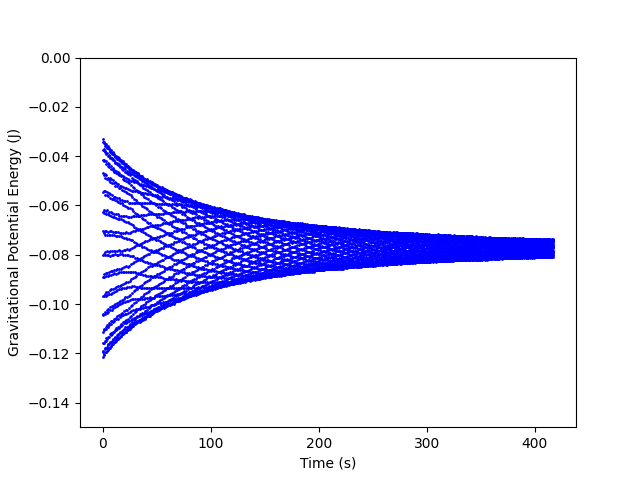
\includegraphics[width=0.5\linewidth]{gravitational-potential-energy}
                    \caption{Gravitational potential energy over time}
                    \label{fig:gravitational-potential-energy}
                \end{figure}
                
                ~One interesting thing to note is that in the gravitational potential energy graph it looks like there are a series of lines at different heights.
                However, this is only a coincidence from the fact that the period of oscillation is extremely close to the measuring interval of the ultrasound motion detector times a certain constant factor, in other words, the period of oscillation is extremely close to a multiple of the measuring interval.
                In this case, the period of the oscillating mass is extremely close to 0.45 seconds.
                When the motion detector measures the position of the mass, the mass is at a similar position to when the motion detector measured exactly one cycle ago, thus the gravitational potential energy looks very similar to a previous point.
                Since this happens for every cycle, the gravitational potential energy graph looks like a series of lines at different heights.
                
                Zooming in on a specific section, such as from 0 to 2.5 seconds, shows how it is actually just a single line oscillating up and down.
                
                %figure gravitational-potential-energy-zoomed
                \begin{figure}[H]
                    \centering
                    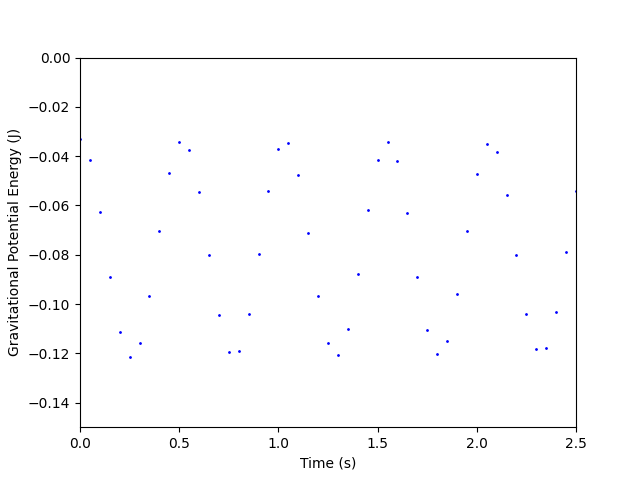
\includegraphics[width=0.5\linewidth]{gravitational-potential-energy-zoomed}
                    \caption{Gravitational potential energy over time (zoomed in on 0 to 2.5 seconds)}
                    \label{fig:gravitational-potential-energy-zoomed}
                \end{figure}
            
            \subsubsection{Calculating spring/elastic potential energy}
                Spring potential energy is the energy stored in a spring when it is stretched or compressed.
                The equation for spring potential energy is $U = \frac{1}{2}k(\Delta x)^2$, where $k$ is the spring constant and $\Delta x$ is the distance the spring is stretched.
                
                \begin{equation}
                    \begin{aligned}
                        U_{\text{s}} &= \frac{1}{2}k(\Delta x)^2 \\
                        U_{\text{s}} &= \frac{1}{2}(10 \frac{\text{ N}}{\text{ m}})(x_0 \text{ m} - x)^2 \\
                        U_{\text{s}} &= \frac{1}{2}(10 \frac{\text{ N}}{\text{ m}})(0.328 \text{ m} - x)^2 \\
                    \end{aligned}\label{eq:spring-potential-energy-equation}
                \end{equation}
                
                Using the data from section~\ref{subsec:change-in-mechanical-energy-over-time-data} and equation~\ref{eq:spring-potential-energy-equation}, we can calculate the spring potential energy for each data point.
                
                %figure elastic-potential-energy
                \begin{figure}[H]
                    \centering
                    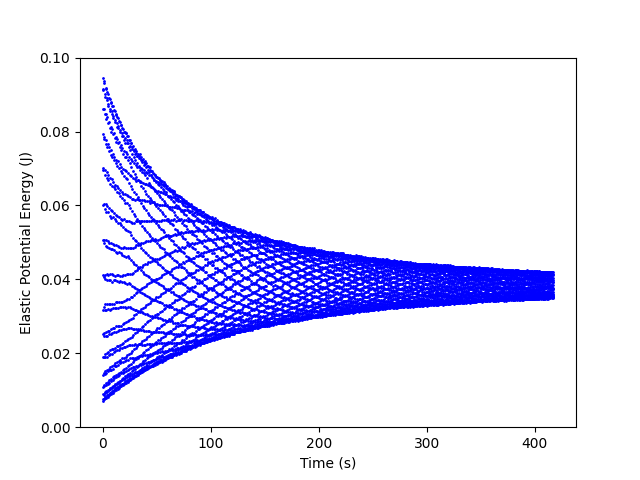
\includegraphics[width=0.5\linewidth]{elastic-potential-energy}
                    \caption{Elastic potential energy over time}
                    \label{fig:elastic-potential-energy}
                \end{figure}
                
                Just like in gravitational potential energy, the elastic potential energy graph looks like a series of lines at different heights.
                However, this is once again a coincidence caused by the period of the oscillating mass being extremely close to a multiple of the measuring interval.
                
                Zooming in on a specific section, such as from 0 to 2.5 seconds, shows how it is actually just a single line oscillating up and down.
                
                %figure elastic-potential-energy-zoomed
                \begin{figure}[H]
                    \centering
                    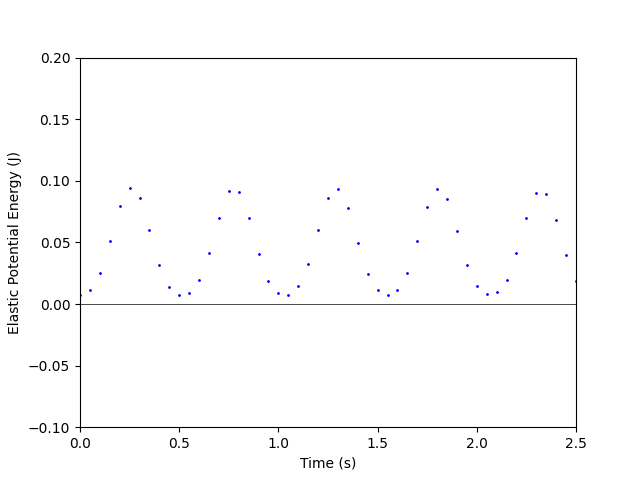
\includegraphics[width=0.5\linewidth]{elastic-potential-energy-zoomed}
                    \caption{Elastic potential energy over time (zoomed in on 0 to 2.5 seconds)}
                    \label{fig:elastic-potential-energy-zoomed}
                \end{figure}
            
            \subsubsection{Calculating kinetic energy}
                
                The kinetic energy of an object is the energy that the object possesses due to its motion.
                The equation for kinetic energy is $K = \frac{1}{2}mv^2$, where $m$ is the mass of the object and $v$ is the velocity of the object.
                
                \begin{equation}
                    \begin{aligned}
                        K &= \frac{1}{2}mv^2 \\
                        K &= \frac{1}{2}(0.09 \text{ kg})(v)^2 \\
                    \end{aligned}\label{eq:kinetic-energy-equation}
                \end{equation}
                
                Using the data from section~\ref{subsec:change-in-mechanical-energy-over-time-data} and equation~\ref{eq:kinetic-energy-equation}, we can calculate the kinetic energy for each data point.
                
                %figure kinetic-energy
                \begin{figure}[H]
                    \centering
                    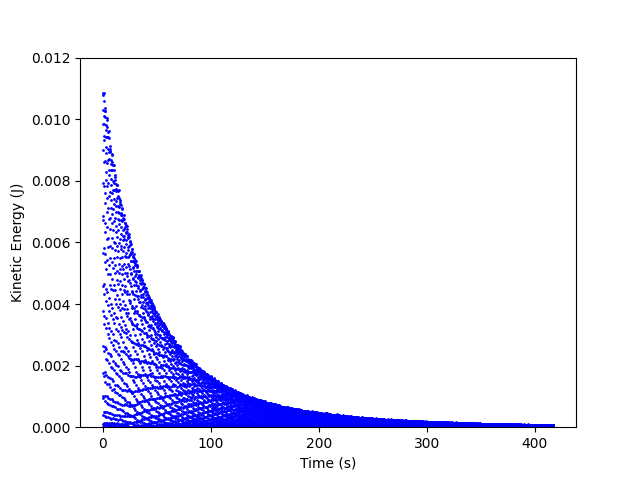
\includegraphics[width=0.5\linewidth]{kinetic-energy}
                    \caption{Kinetic energy over time}
                    \label{fig:kinetic-energy}
                \end{figure}
                
                Just like in gravitational potential energy and elastic potential energy, the kinetic energy graph looks like a series of lines at different heights.
                However, this is once again a coincidence caused by the period of the oscillating mass being extremely close to a multiple of the measuring interval.
                
                Zooming in on a specific section, such as from 0 to 1 second, shows how it is actually just a single line oscillating up and down.
                
                %figure kinetic-energy-zoomed
                \begin{figure}[H]
                    \centering
                    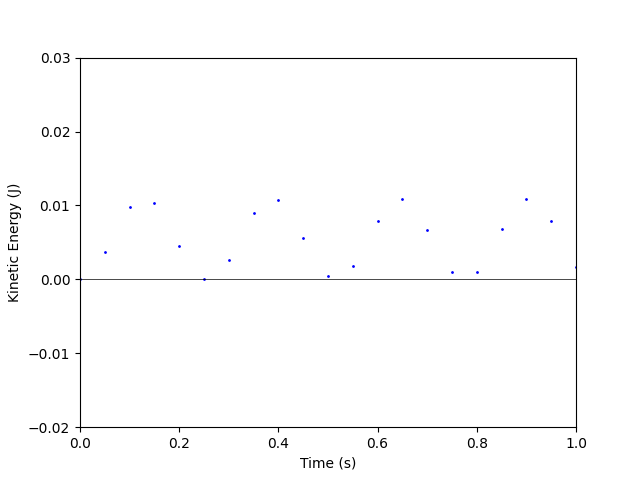
\includegraphics[width=0.5\linewidth]{kinetic-energy-zoomed}
                    \caption{Kinetic energy over time (zoomed in on 0 to 1 second)}
                    \label{fig:kinetic-energy-zoomed}
                \end{figure}
            
            \subsubsection{Calculating mechanical energy}
                Mechanical energy is the sum of kinetic energy and potential energy.
                The equation for mechanical energy is $M = U + K$, where $M$ is the mechanical energy, $U$ is the potential energy, and $K$ is the kinetic energy.
                Since potential energy consists of two different forms of energy, gravitational potential energy and spring potential energy, the equation for mechanical energy can be rewritten as follows:
                
                \begin{equation}
                    \begin{aligned}
                        \notag
                        M &= U + K \\
                        M &= U_{\text{gravitational}} + U_{\text{spring}} + K \\
                        M &= U_{\text{g}} + U_{\text{s}} + K \\
                    \end{aligned}\label{eq:mechanical-energy-equation}
                \end{equation}
                
                Using the data from section~\ref{subsec:change-in-mechanical-energy-over-time-data} and equations~\ref{eq:gravitational-potential-energy-equation},~\ref{eq:spring-potential-energy-equation}, and~\ref{eq:kinetic-energy-equation}, we can calculate the mechanical energy for each data point.
                
                %figure mechanical-energy
                \begin{figure}[H]
                    \centering
                    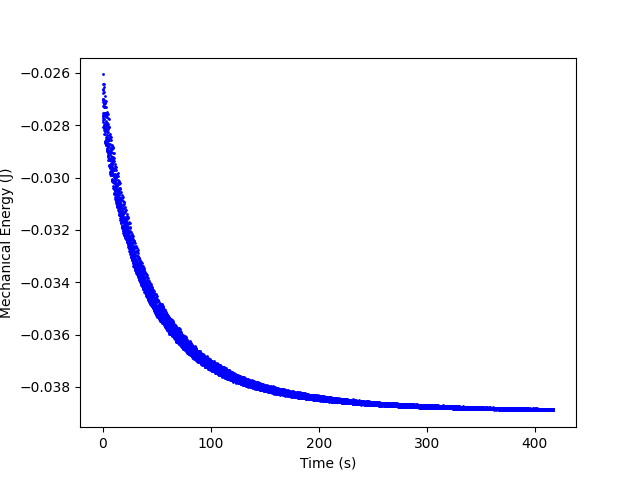
\includegraphics[width=0.5\linewidth]{mechanical-energy}
                    \caption{Mechanical energy over time}
                    \label{fig:mechanical-energy}
                \end{figure}
                
                In this case, mechanical energy is negative because gravitational potential energy is more negative than the sum of spring potential energy and kinetic energy.
                This is because gravitational potential energy only has meaning when compared over time.
        
        \subsection{Calculating the change in mechanical energy over time}
            Since potential energy is relevant only when compared over time, and since the mechanical energy is the sum of potential energy and kinetic energy, the mechanical energy is also only relevant as a change, i.e. compared over time.
            
            %todo do i talk about how it should be stairstep or do i just fit a graph?
            
            If we look between $t=0$ seconds and $t=10$ seconds, we can see that the mechanical energy is decreasing.
            If we take the average mechanical energy of the first cycle and the average mechanical energy of the last cycle, we can determine the rate of change of mechanical energy over time at around $t = 5$ seconds.
            
            
            The following data is the time, position, velocity, and mechanical energy of the points on the first cycle:
%0.00 0.291 -0.006 -0.026
%0.05 0.281 -0.289 -0.027
%0.10 0.257 -0.467 -0.028
%0.15 0.227 -0.478 -0.028
%0.20 0.202 -0.319 -0.027
%0.25 0.191 -0.046 -0.027
%0.30 0.197 0.243 -0.027
%0.35 0.218 0.447 -0.028
%0.40 0.248 0.490 -0.028
%0.45 0.275 0.354 -0.027
%0.50 0.289 0.094 -0.026
            
            %table of data
            \begin{table}[H]
                \centering
                \begin{tabular}{|c|c|c|c|}
                    \hline
                    Time [s] & Position [m] & Velocity [m/s] & Mechanical Energy [J] \\
                    \hline
                    0.00     & 0.291        & -0.006         & -0.026                \\
                    \hline
                    0.05     & 0.281        & -0.289         & -0.027                \\
                    \hline
                    0.10     & 0.257        & -0.467         & -0.028                \\
                    \hline
                    0.15     & 0.227        & -0.478         & -0.028                \\
                    \hline
                    0.20     & 0.202        & -0.319         & -0.027                \\
                    \hline
                    0.25     & 0.191        & -0.046         & -0.027                \\
                    \hline
                    0.30     & 0.197        & 0.243          & -0.027                \\
                    \hline
                    0.35     & 0.218        & 0.447          & -0.028                \\
                    \hline
                    0.40     & 0.248        & 0.490          & -0.028                \\
                    \hline
                    0.45     & 0.275        & 0.354          & -0.027                \\
                    \hline
                    0.50     & 0.289        & 0.094          & -0.026                \\
                    \hline
                \end{tabular} %todo does it matter that its slightly more than 1 cycle
                \caption{Data for the first cycle}\label{tab:first-cycle-mechanical-energy-table}
            \end{table}
            
            We can then take the average of the mechanical energy for the first cycle as follows using the data from table~\ref{tab:first-cycle-mechanical-energy-table}:
            
            \begin{equation}
                \begin{aligned}
                    M_{\text{avg, 0}} &= \frac{M_1 + M_2 + M_3 + M_4 + M_5 + M_6 + M_7 + M_8 + M_9 + M_{10} + M_{11}}{11} \\
                    M_{\text{avg, 0}} &= \frac{-0.026 -0.027 -0.028 -0.028 -0.027 -0.027 -0.027 -0.028 -0.028 -0.027 -0.026}{11} \\
                    M_{\text{avg, 0}} &= -0.027 \text{ J} \\
                \end{aligned}\label{eq:average-mechanical-energy-first-cycle}
            \end{equation}
            
            Similarly, we can analyze the last cycle before 10 seconds, the following data is the time, position, velocity, and mechanical energy of the points on the last cycle before 10 seconds:
            %9.30 0.285 -0.010 -0.029
            %9.35 0.276 -0.259 -0.029
            %9.40 0.255 -0.414 -0.030
            %9.45 0.228 -0.422 -0.030
            %9.50 0.206 -0.280 -0.030
            %9.55 0.196 -0.037 -0.029
            %9.60 0.202 0.219 -0.030
            %9.65 0.221 0.397 -0.030
            %9.70 0.248 0.435 -0.030
            %9.75 0.272 0.315 -0.029
            %9.80 0.284 0.080 -0.029
            %9.85 0.281 -0.182 -0.029
            
            %table of data
            \begin{table}[H]
                \centering
                \begin{tabular}{|c|c|c|c|}
                    \hline
                    Time [s] & Position [m] & Velocity [m/s] & Mechanical Energy [J] \\
                    \hline
                    9.30     & 0.285        & -0.010         & -0.029                \\
                    \hline
                    9.35     & 0.276        & -0.259         & -0.029                \\
                    \hline
                    9.40     & 0.255        & -0.414         & -0.030                \\
                    \hline
                    9.45     & 0.228        & -0.422         & -0.030                \\
                    \hline
                    9.50     & 0.206        & -0.280         & -0.030                \\
                    \hline
                    9.55     & 0.196        & -0.037         & -0.029                \\
                    \hline
                    9.60     & 0.202        & 0.219          & -0.030                \\
                    \hline
                    9.65     & 0.221        & 0.397          & -0.030                \\
                    \hline
                    9.70     & 0.248        & 0.435          & -0.030                \\
                    \hline
                    9.75     & 0.272        & 0.315          & -0.029                \\
                    \hline
                    9.80     & 0.284        & 0.080          & -0.029                \\
                    \hline
                    9.85     & 0.281        & -0.182         & -0.029                \\
                    \hline
                \end{tabular} %todo does it matter that its slightly more than 1 cycle
                \caption{Data for the last cycle before 10 seconds}\label{tab:last-cycle-before-10-seconds-mechanical-energy-table}
            \end{table}
            
            Using the data in table~\ref{tab:last-cycle-before-10-seconds-mechanical-energy-table}, we can calculate the average mechanical energy of the last cycle before 10 seconds as follows:
            
            \begin{equation}
                \begin{aligned}
                    M_{\text{avg, 9.3}} &= \frac{M_1 + M_2 + M_3 + M_4 + M_5 + M_6 + M_7 + M_8 + M_9 + M_{10} + M_{11} + M_{12}}{12} \\
                    M_{\text{avg, 9.3}} &= \frac{-0.029 -0.029 -0.030 -0.030 -0.030 -0.029 -0.030 -0.030 -0.030 -0.029 -0.029 -0.029}{12} \\
                    M_{\text{avg, 9.3}} &= -0.030 \text{ J} \\
                \end{aligned}\label{eq:average-mechanical-energy-last-cycle-before-10-seconds}
            \end{equation}
            
            Therefore, using the data from equation~\ref{eq:average-mechanical-energy-first-cycle} and equation~\ref{eq:average-mechanical-energy-last-cycle-before-10-seconds}, we can calculate the rate of change of mechanical energy over time at around $t = 5$ seconds as follows:
            
            \begin{equation}
                \begin{aligned}
                    \frac{\Delta M}{\Delta t} &= \frac{M_{\text{avg, 9.3}} - M_{\text{avg, 0}}}{9.3 \text{ s} - 0 \text{ s}} \\
                    \frac{\Delta M}{\Delta t} &= \frac{-0.030 \text{ J} - (-0.027 \text{ J})}{9.3 \text{ s} - 0 \text{ s}} \\
                    \frac{\Delta M}{\Delta t} &= \frac{-0.003 \text{ J}}{9.3 \text{ s}} \\
                    \frac{\Delta M}{\Delta t} &= -0.000322 \frac{\text{ J}}{\text{ s}} \\
                \end{aligned}\label{eq:rate-of-change-of-mechanical-energy-over-time}
            \end{equation}
            
            Therefore, the rate of change of mechanical energy over time at around $t = 5$ seconds is $-0.000322 \frac{\text{ J}}{\text{ s}}$. \\
%            Using this information, we can graph a line of best fit for the change in mechanical energy over time.
            \newline \indent The following is the mechanical energy for the cycle around $t=5$ seconds:
%            4.65 0.287 -0.010 -0.028
%4.70 0.278 -0.274 -0.028
%4.75 0.256 -0.439 -0.029
%4.80 0.228 -0.448 -0.029
%4.85 0.204 -0.297 -0.029
%4.90 0.194 -0.040 -0.028
%4.95 0.200 0.231 -0.029
%5.00 0.220 0.420 -0.029
%5.05 0.248 0.458 -0.029
%5.10 0.273 0.333 -0.028
%5.15 0.286 0.087 -0.028
            
            %table of data
            \begin{table}[H]
                \centering
                \begin{tabular}{|c|c|c|c|}
                    \hline
                    Time [s] & Position [m] & Velocity [m/s] & Mechanical Energy [J] \\
                    \hline
                    4.65     & 0.287        & -0.010         & -0.028                \\
                    \hline
                    4.70     & 0.278        & -0.274         & -0.028                \\
                    \hline
                    4.75     & 0.256        & -0.439         & -0.029                \\
                    \hline
                    4.80     & 0.228        & -0.448         & -0.029                \\
                    \hline
                    4.85     & 0.204        & -0.297         & -0.029                \\
                    \hline
                    4.90     & 0.194        & -0.040         & -0.028                \\
                    \hline
                    4.95     & 0.200        & 0.231          & -0.029                \\
                    \hline
                    5.00     & 0.220        & 0.420          & -0.029                \\
                    \hline
                    5.05     & 0.248        & 0.458          & -0.029                \\
                    \hline
                    5.10     & 0.273        & 0.333          & -0.028                \\
                    \hline
                    5.15     & 0.286        & 0.087          & -0.028                \\
                    \hline
                \end{tabular} %todo does it matter that its slightly more than 1 cycle
                \caption{Data for the cycle around $t=5$ seconds}\label{tab:cycle-around-5-seconds-mechanical-energy-table}
            \end{table}
            
            Using the data from table~\ref{tab:cycle-around-5-seconds-mechanical-energy-table} we can calculate the average mechanical energy of the cycle around $t=5$ seconds as follows:
            \begin{equation}
                \begin{aligned}
                    M_{\text{avg, 5}} &= \frac{M_1 + M_2 + M_3 + M_4 + M_5 + M_6 + M_7 + M_8 + M_9 + M_{10} + M_{11}}{11} \\
                    M_{\text{avg, 5}} &= \frac{-0.028 -0.028 -0.029 -0.029 -0.029 -0.028 -0.029 -0.029 -0.029 -0.028 -0.028}{11} \\
                    M_{\text{avg, 5}} &= -0.028 \text{ J} \\
                \end{aligned}\label{eq:average-mechanical-energy-cycle-around-5-seconds}
            \end{equation}
            
            Using the data from table~\ref{tab:first-cycle-mechanical-energy-table}, table~\ref{tab:last-cycle-before-10-seconds-mechanical-energy-table}, and table~\ref{tab:cycle-around-5-seconds-mechanical-energy-table}, we can graph a linear best fit line for the change in mechanical energy over time for the change in mechanical energy around $t = 5$ seconds.
            
            To find the equation of the line of best fit, we can use the following equation:
            \begin{equation}
                \begin{aligned}
                    y &= mx + b \\
                    y &= \frac{\Delta M}{\Delta t}x + b \\
                \end{aligned}\label{eq:line-of-best-fit-equation}
            \end{equation}
            
            Since we have already calculated $\frac{\Delta M}{\Delta t}$ in equation~\ref{eq:rate-of-change-of-mechanical-energy-over-time}, and we can use the point at $t = 5$ seconds with the mechanical energy from equation~\ref{eq:average-mechanical-energy-cycle-around-5-seconds}, we can calculate $b$ as follows using equation~\ref{eq:line-of-best-fit-equation}:
            
            \begin{equation}
                \begin{aligned}
                    b &= y - \frac{\Delta M}{\Delta t}x \\
                    b &= y - \frac{\Delta M}{\Delta t}x \\
                    b &= -0.028 \text{ J} - (-0.000322 \frac{\text{ J}}{\text{ s}})(5 \text{ s}) \\
                    b &= -0.026 \text{ J} \\
                \end{aligned}\label{eq:line-of-best-fit-b}
            \end{equation}
            
            Using $\Delta M = y$ and $\Delta t = x$ from equation~\ref{eq:rate-of-change-of-mechanical-energy-over-time}, and $b$ from equation~\ref{eq:line-of-best-fit-b}, we can calculate the equation of the line of best fit around $t=5$ seconds as follows:
            
            \begin{equation}
                \begin{aligned}
                    y &= mx + b \\
                    y &= \frac{\Delta M}{\Delta t}x + b \\
                    y &= -0.000322 \frac{\text{ J}}{\text{ s}}x - 0.026 \text{ J} \\
                \end{aligned}\label{eq:line-of-best-fit-equation-around-5-seconds}
            \end{equation}
            
            This can be visualized on the graph as shown below:
            
            %figure mechanical-energy-linear-fit-5s
            \begin{figure}[H]
                \centering
                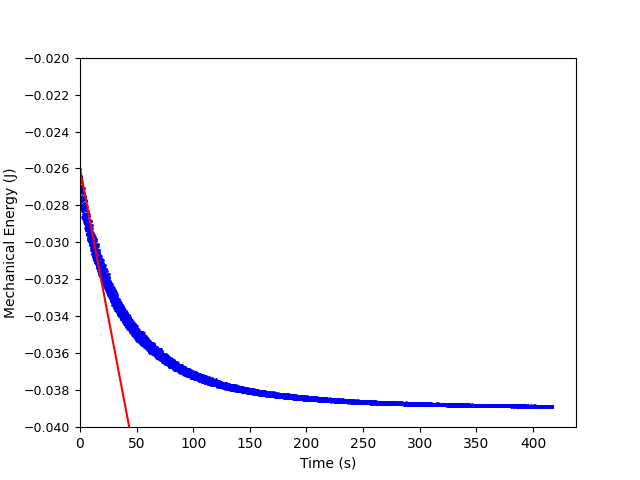
\includegraphics[width=0.5\linewidth]{mechanical-energy-linear-fit-5s}
                \caption{Mechanical energy over time with linear fit around $t=5$ seconds}
                \label{fig:mechanical-energy-linear-fit-5s}
            \end{figure}
            
            On this graph it is possible to see that even though the line of best fit is relatively accurate for the first 30 to 50 seconds, it rapidly does not become accurate due to the fact that the rate of change of mechanical energy over time is not constant.
            
            To best demonstrate that we can calculate the linear line of best fit for 2 more position on the graph, the first one around $t=100$ seconds, and the second one around $t=300$ seconds.\\
            \newline \indent Now to calculate the linear line of best fit around $t=100$ seconds, we will use the cycle following $t=75$ seconds, the cycle that includes $t=100$ seconds, and the cycle before $t=125$ seconds.
            
            The following table contains the mechanical energy data for the cycle after $t=75$ seconds:
%            75.40 0.264 -0.008 -0.0361
%75.45 0.259 -0.139 -0.0362
%75.50 0.248 -0.220 -0.0365
%75.55 0.234 -0.222 -0.0366
%75.60 0.222 -0.144 -0.0365
%75.65 0.217 -0.014 -0.0364
%75.70 0.221 0.120 -0.0365
%75.75 0.231 0.211 -0.0366
%75.80 0.245 0.227 -0.0365
%75.85 0.257 0.162 -0.0363
%75.90 0.264 0.038 -0.0360
            
            %table of data
            \begin{table}[H]
                \centering
                \begin{tabular}{|c|c|c|c|}
                    \hline
                    Time [s] & Position [m] & Velocity [m/s] & Mechanical Energy [J] \\
                    \hline
                    75.40    & 0.264        & -0.008         & -0.0361               \\
                    \hline
                    75.45    & 0.259        & -0.139         & -0.0362               \\
                    \hline
                    75.50    & 0.248        & -0.220         & -0.0365               \\
                    \hline
                    75.55    & 0.234        & -0.222         & -0.0366               \\
                    \hline
                    75.60    & 0.222        & -0.144         & -0.0365               \\
                    \hline
                    75.65    & 0.217        & -0.014         & -0.0364               \\
                    \hline
                    75.70    & 0.221        & 0.120          & -0.0365               \\
                    \hline
                    75.75    & 0.231        & 0.211          & -0.0366               \\
                    \hline
                    75.80    & 0.245        & 0.227          & -0.0365               \\
                    \hline
                    75.85    & 0.257        & 0.162          & -0.0363               \\
                    \hline
                    75.90    & 0.264        & 0.038          & -0.0360               \\
                    \hline
                \end{tabular} %todo does it matter that its slightly more than 1 cycle
                \caption{Data for the cycle at $t=75$ seconds}\label{tab:cycle-at-75-seconds-mechanical-energy-table}
            \end{table}
            
            Using the data from table~\ref{tab:cycle-at-75-seconds-mechanical-energy-table}, we can calculate the average mechanical energy of the cycle at $t=75$ seconds as follows:
            
            \begin{equation}
                \begin{aligned}
                    M_{\text{avg, 75}} &= \frac{M_1 + M_2 + M_3 + M_4 + M_5 + M_6 + M_7 + M_8 + M_9 + M_{10} + M_{11}}{11} \\
                    M_{\text{avg, 75}} &= \frac{-0.0361 -0.0362 -0.0365 -0.0366 -0.0365 -0.0364 -0.0365 -0.0366 -0.0365 -0.0363 -0.0360}{11} \\
                    M_{\text{avg, 75}} &= -0.0364 \text{ J} \\
                \end{aligned}\label{eq:average-mechanical-energy-cycle-at-75-seconds}
            \end{equation}
            
            The following table contains the mechanical energy data for the cycle at $t=100$ seconds:
%            99.65 0.260 0.020 -0.0369
%99.70 0.257 -0.093 -0.0370
%99.75 0.249 -0.172 -0.0372
%99.80 0.237 -0.189 -0.0373
%99.85 0.227 -0.137 -0.0373
%99.90 0.222 -0.038 -0.0372
%99.95 0.223 0.075 -0.0373
%100.00 0.230 0.162 -0.0373
%100.05 0.241 0.192 -0.0373
%100.10 0.252 0.151 -0.0371
%100.15 0.259 0.055 -0.0370
            
            %table of data
            \begin{table}[H]
                \centering
                \begin{tabular}{|c|c|c|c|}
                    \hline
                    Time [s] & Position [m] & Velocity [m/s] & Mechanical Energy [J] \\
                    \hline
                    99.65    & 0.260        & 0.020          & -0.0369               \\
                    \hline
                    99.70    & 0.257        & -0.093         & -0.0370               \\
                    \hline
                    99.75    & 0.249        & -0.172         & -0.0372               \\
                    \hline
                    99.80    & 0.237        & -0.189         & -0.0373               \\
                    \hline
                    99.85    & 0.227        & -0.137         & -0.0373               \\
                    \hline
                    99.90    & 0.222        & -0.038         & -0.0372               \\
                    \hline
                    99.95    & 0.223        & 0.075          & -0.0373               \\
                    \hline
                    100.00   & 0.230        & 0.162          & -0.0373               \\
                    \hline
                    100.05   & 0.241        & 0.192          & -0.0373               \\
                    \hline
                    100.10   & 0.252        & 0.151          & -0.0371               \\
                    \hline
                    100.15   & 0.259        & 0.055          & -0.0370               \\
                    \hline
                \end{tabular} %todo does it matter that its slightly more than 1 cycle
                \caption{Data for the cycle at $t=100$ seconds}\label{tab:cycle-at-100-seconds-mechanical-energy-table}
            \end{table}
            
            Using the data from table~\ref{tab:cycle-at-100-seconds-mechanical-energy-table}, we can calculate the average mechanical energy of the cycle at $t=100$ seconds as follows:
            
            \begin{equation}
                \begin{aligned}
                    M_{\text{avg, 100}} &= \frac{M_1 + M_2 + M_3 + M_4 + M_5 + M_6 + M_7 + M_8 + M_9 + M_{10} + M_{11}}{11} \\
                    M_{\text{avg, 100}} &= \frac{-0.0369 -0.0370 -0.0372 -0.0373 -0.0373 -0.0372 -0.0373 -0.0373 -0.0373 -0.0371 -0.0370}{11} \\
                    M_{\text{avg, 100}} &= -0.0372 \text{ J} \\
                \end{aligned}\label{eq:average-mechanical-energy-cycle-at-100-seconds}
            \end{equation}
            
            The following table contains the mechanical energy data for the cycle before $t=125$ seconds:
%            124.45 0.256 -0.032 -0.0375
%124.50 0.251 -0.116 -0.0377
%124.55 0.243 -0.158 -0.0378
%124.60 0.233 -0.144 -0.0378
%124.65 0.226 -0.078 -0.0378
%124.70 0.224 0.016 -0.0377
%124.75 0.228 0.104 -0.0378
%124.80 0.236 0.156 -0.0378
%124.85 0.246 0.151 -0.0377
%124.90 0.254 0.090 -0.0376
%124.95 0.256 -0.002 -0.0376
            
            %table of data
            \begin{table}[H]
                \centering
                \begin{tabular}{|c|c|c|c|}
                    \hline
                    Time [s] & Position [m] & Velocity [m/s] & Mechanical Energy [J] \\
                    \hline
                    124.45   & 0.256        & -0.032         & -0.0375               \\
                    \hline
                    124.50   & 0.251        & -0.116         & -0.0377               \\
                    \hline
                    124.55   & 0.243        & -0.158         & -0.0378               \\
                    \hline
                    124.60   & 0.233        & -0.144         & -0.0378               \\
                    \hline
                    124.65   & 0.226        & -0.078         & -0.0378               \\
                    \hline
                    124.70   & 0.224        & 0.016          & -0.0377               \\
                    \hline
                    124.75   & 0.228        & 0.104          & -0.0378               \\
                    \hline
                    124.80   & 0.236        & 0.156          & -0.0378               \\
                    \hline
                    124.85   & 0.246        & 0.151          & -0.0377               \\
                    \hline
                    124.90   & 0.254        & 0.090          & -0.0376               \\
                    \hline
                    124.95   & 0.256        & -0.002         & -0.0376               \\
                    \hline
                \end{tabular} %todo does it matter that its slightly more than 1 cycle
                \caption{Data for the cycle at $t=125$ seconds}\label{tab:cycle-at-125-seconds-mechanical-energy-table}
            
            \end{table}
            
            Using the data from table~\ref{tab:cycle-at-100-seconds-mechanical-energy-table}, we can calculate the average mechanical energy of the cycle at $t=125$ seconds as follows:
            
            \begin{equation}
                \begin{aligned}
                    M_{\text{avg, 125}} &= \frac{M_1 + M_2 + M_3 + M_4 + M_5 + M_6 + M_7 + M_8 + M_9 + M_{10} + M_{11}}{11} \\
                    M_{\text{avg, 125}} &= \frac{-0.0375 -0.0377 -0.0378 -0.0378 -0.0378 -0.0377 -0.0378 -0.0378 -0.0377 -0.0376 -0.0376}{11} \\
                    M_{\text{avg, 125}} &= -0.0377 \text{ J} \\
                \end{aligned}\label{eq:average-mechanical-energy-cycle-at-125-seconds}
            \end{equation}
            
            Now that we have the average mechanical energy for the cycle before $t=125$ seconds, the cycle at $t=100$ seconds, and the cycle after $t=75$ seconds, we can calculate the rate of change of mechanical energy over time at around $t=100$ seconds as follows:
            
            
            \begin{equation}
                \begin{aligned}
                    \frac{\Delta M}{\Delta t} &= \frac{M_{\text{avg, 125}} - M_{\text{avg, 75}}} {125 \text{ s} - 75 \text{ s}} \\
                    \frac{\Delta M}{\Delta t} &= \frac{-0.0377 \text{ J} - (-0.0364 \text{ J})} {125 \text{ s} - 75 \text{ s}} \\
                    \frac{\Delta M}{\Delta t} &= \frac{-0.0013 \text{ J}} {50 \text{ s}} \\
                    \frac{\Delta M}{\Delta t} &= -0.000026 \frac{\text{ J}}{\text{ s}} \\
                \end{aligned}\label{eq:rate-of-change-of-mechanical-energy-over-time-around-100-seconds}
            \end{equation}
            
            
            Therefore, the rate of change of mechanical energy over time at around $t=100$ seconds is $-0.000026 \frac{\text{ J}}{\text{ s}}$. \\
            
            Using this information, we can calculate the equation of the line of best fit around $t=100$ seconds as follows:
            
            \begin{equation}
                \begin{aligned}
                    y &= mx + b \\
                    y &= \frac{\Delta M}{\Delta t}x + b \\
                    y &= -0.000026 \frac{\text{ J}}{\text{ s}}x + b \\
                \end{aligned}\label{eq:line-of-best-fit-equation-around-100-seconds-w/ob}
            \end{equation}
            
            Since we have already calculated $\frac{\Delta M}{\Delta t}$ in equation~\ref{eq:rate-of-change-of-mechanical-energy-over-time-around-100-seconds}, and we can use the point at $t = 100$ seconds with the mechanical energy from equation~\ref{eq:average-mechanical-energy-cycle-at-100-seconds}, we can calculate $b$ as follows using equation~\ref{eq:line-of-best-fit-equation-around-100-seconds-w/ob}:
            
            \begin{equation}
                \begin{aligned}
                    b &= y - \frac{\Delta M}{\Delta t}x \\
                    b &= y - \frac{\Delta M}{\Delta t}x \\
                    b &= -0.0372 \text{ J} - (-0.000026 \frac{\text{ J}}{\text{ s}})(100 \text{ s}) \\
                    b &= -0.0346 \text{ J} \\
                \end{aligned}\label{eq:line-of-best-fit-b-around-100-seconds}
            \end{equation}
            
            Using $\Delta M = y$ and $\Delta t = x$ from equation~\ref{eq:rate-of-change-of-mechanical-energy-over-time-around-100-seconds}, and $b$ from equation~\ref{eq:line-of-best-fit-b-around-100-seconds}, we can calculate the equation of the line of best fit around $t=100$ seconds as follows:
            
            \begin{equation}
                \begin{aligned}
                    y &= mx + b \\
                    y &= \frac{\Delta M}{\Delta t}x + b \\
                    y &= -0.000026 \frac{\text{ J}}{\text{ s}}x - 0.0346 \text{ J} \\
                \end{aligned}\label{eq:line-of-best-fit-equation-around-100-seconds}
            \end{equation}
            
            If we graph that line of best fit on the graph of mechanical energy, we get the following graph:
            
            %figure mechanical-energy-linear-fit-100s
            \begin{figure}[H]
                \centering
                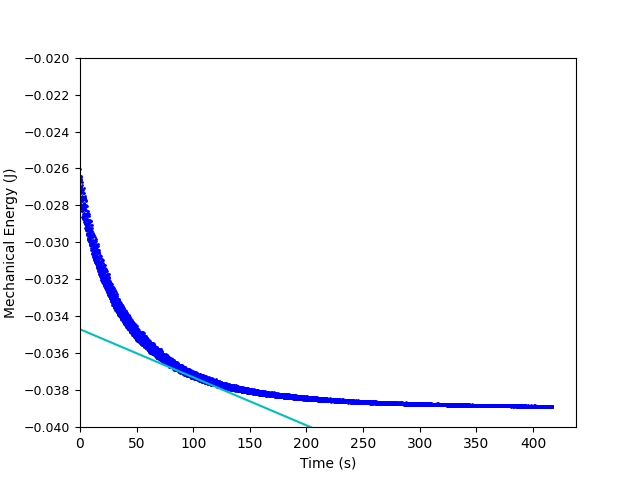
\includegraphics[width=0.5\linewidth]{mechanical-energy-linear-fit-100s}
                \caption{Mechanical energy over time with linear fit around $t=100$ seconds}
                \label{fig:mechanical-energy-linear-fit-100s}
            \end{figure}
            
            On this graph, even though this linear line of best fit is relatively accurate around $t=100$ seconds, it is not accurate for the rest of the graph, due to the fact that the rate of change of mechanical energy over time is not constant. In fact, as soon as the time is greater than $t=125$ seconds or less than $t=75$ seconds, the line of best fit is already significantly inaccurate.
            
            The last line of best fit that we will calculate is the one around $t=300$ seconds. To calculate this line of best fit, we will use the cycle after $t=250$ seconds, the cycle that includes $t=300$ seconds, and the cycle before $t=350$ seconds.
            
            The following table contains the mechanical energy data for the cycle after $t=250$ seconds:
%            250.35 0.248 0.002 -0.03858
%250.40 0.247 -0.045 -0.03860
%250.45 0.243 -0.075 -0.03864
%250.50 0.238 -0.076 -0.03867
%250.55 0.234 -0.051 -0.03868
%250.60 0.232 -0.008 -0.03868
%250.65 0.233 0.041 -0.03866
%250.70 0.237 0.073 -0.03868
%250.75 0.242 0.077 -0.03866
%250.80 0.246 0.055 -0.03862
%250.85 0.248 0.013 -0.03859
            
            %table of data
            \begin{table}[H]
                \centering
                \begin{tabular}{|c|c|c|c|}
                    \hline
                    Time [s] & Position [m] & Velocity [m/s] & Mechanical Energy [J] \\
                    \hline
                    250.35   & 0.248        & 0.002          & -0.03858              \\
                    \hline
                    250.40   & 0.247        & -0.045         & -0.03860              \\
                    \hline
                    250.45   & 0.243        & -0.075         & -0.03864              \\
                    \hline
                    250.50   & 0.238        & -0.076         & -0.03867              \\
                    \hline
                    250.55   & 0.234        & -0.051         & -0.03868              \\
                    \hline
                    250.60   & 0.232        & -0.008         & -0.03868              \\
                    \hline
                    250.65   & 0.233        & 0.041          & -0.03866              \\
                    \hline
                    250.70   & 0.237        & 0.073          & -0.03868              \\
                    \hline
                    250.75   & 0.242        & 0.077          & -0.03866              \\
                    \hline
                    250.80   & 0.246        & 0.055          & -0.03862              \\
                    \hline
                    250.85   & 0.248        & 0.013          & -0.03859              \\
                    \hline
                \end{tabular} %todo does it matter that its slightly more than 1 cycle
                \caption{Data for the cycle at $t=250$ seconds}\label{tab:cycle-at-250-seconds-mechanical-energy-table}
            \end{table}
            
            Using the data from table~\ref{tab:cycle-at-250-seconds-mechanical-energy-table}, we can calculate the average mechanical energy of the cycle at $t=250$ seconds as follows:
            
            \begin{equation}
                \begin{aligned}
                    M_{\text{avg, 250}} &= \frac{M_1 + M_2 + M_3 + M_4 + M_5 + M_6 + M_7 + M_8 + M_9 + M_{10} + M_{11}}{11} \\
                    M_{\text{avg, 250}} &= \frac{-0.03858 -0.03860 -0.03864 -  \ldots -0.03866 -0.03862 -0.03859}{11} \\
                    M_{\text{avg, 250}} &= -0.03865 \text{ J} \\
                \end{aligned}\label{eq:average-mechanical-energy-cycle-at-250-seconds}
            \end{equation}
            
            The following table contains the mechanical energy data for the cycle at $t=300$ seconds:
%            299.90 0.247 -0.015 -0.03870
%299.95 0.245 -0.047 -0.03873
%300.00 0.241 -0.061 -0.03877
%300.05 0.238 -0.054 -0.03879
%300.10 0.235 -0.030 -0.03879
%300.15 0.234 0.006 -0.03879
%300.20 0.236 0.040 -0.03879
%300.25 0.239 0.060 -0.03878
%300.30 0.243 0.059 -0.03876
%300.35 0.245 0.038 -0.03872
%300.40 0.247 0.002 -0.03869
            
            %table of data
            \begin{table}[H]
                \centering
                \begin{tabular}{|c|c|c|c|}
                    \hline
                    Time [s] & Position [m] & Velocity [m/s] & Mechanical Energy [J] \\
                    \hline
                    299.90   & 0.247        & -0.015         & -0.03870              \\
                    \hline
                    299.95   & 0.245        & -0.047         & -0.03873              \\
                    \hline
                    300.00   & 0.241        & -0.061         & -0.03877              \\
                    \hline
                    300.05   & 0.238        & -0.054         & -0.03879              \\
                    \hline
                    300.10   & 0.235        & -0.030         & -0.03879              \\
                    \hline
                    300.15   & 0.234        & 0.006          & -0.03879              \\
                    \hline
                    300.20   & 0.236        & 0.040          & -0.03879              \\
                    \hline
                    300.25   & 0.239        & 0.060          & -0.03878              \\
                    \hline
                    300.30   & 0.243        & 0.059          & -0.03876              \\
                    \hline
                    300.35   & 0.245        & 0.038          & -0.03872              \\
                    \hline
                    300.40   & 0.247        & 0.002          & -0.03869              \\
                    \hline
                \end{tabular} %todo does it matter that its slightly more than 1 cycle
                \caption{Data for the cycle at $t=300$ seconds}\label{tab:cycle-at-300-seconds-mechanical-energy-table}
            \end{table}
            
            Using the data from table~\ref{tab:cycle-at-300-seconds-mechanical-energy-table}, we can calculate the average mechanical energy of the cycle at $t=300$ seconds as follows:
            
            \begin{equation}
                \begin{aligned}
                    M_{\text{avg, 300}} &= \frac{M_1 + M_2 + M_3 + M_4 + M_5 + M_6 + M_7 + M_8 + M_9 + M_{10} + M_{11}}{11} \\
                    M_{\text{avg, 300}} &= \frac{-0.03870 -0.03873 -0.03877 -  \ldots -0.03876 -0.03872 -0.03869}{11} \\
                    M_{\text{avg, 300}} &= -0.03876 \text{ J} \\
                \end{aligned}\label{eq:average-mechanical-energy-cycle-at-300-seconds}
            \end{equation}
            
            The following table contains the mechanical energy data for the cycle before $t=350$ seconds:
%            349.40 0.245 0.007 -0.03879
%349.45 0.245 -0.024 -0.03879
%349.50 0.243 -0.045 -0.03882
%349.55 0.240 -0.050 -0.03884
%349.60 0.237 -0.037 -0.03884
%349.65 0.235 -0.011 -0.03885
%349.70 0.236 0.018 -0.03885
%349.75 0.238 0.040 -0.03885
%349.80 0.240 0.049 -0.03884
%349.85 0.243 0.040 -0.03882
%349.90 0.245 0.017 -0.03880
%349.95 0.245 -0.011 -0.03880
            
            %table of data
            \begin{table}[H]
                \centering
                \begin{tabular}{|c|c|c|c|}
                    \hline
                    Time [s] & Position [m] & Velocity [m/s] & Mechanical Energy [J] \\
                    \hline
                    349.40   & 0.245        & 0.007          & -0.03879              \\
                    \hline
                    349.45   & 0.245        & -0.024         & -0.03879              \\
                    \hline
                    349.50   & 0.243        & -0.045         & -0.03882              \\
                    \hline
                    349.55   & 0.240        & -0.050         & -0.03884              \\
                    \hline
                    349.60   & 0.237        & -0.037         & -0.03884              \\
                    \hline
                    349.65   & 0.235        & -0.011         & -0.03885              \\
                    \hline
                    349.70   & 0.236        & 0.018          & -0.03885              \\
                    \hline
                    349.75   & 0.238        & 0.040          & -0.03885              \\
                    \hline
                    349.80   & 0.240        & 0.049          & -0.03884              \\
                    \hline
                    349.85   & 0.243        & 0.040          & -0.03882              \\
                    \hline
                    349.90   & 0.245        & 0.017          & -0.03880              \\
                    \hline
                    349.95   & 0.245        & -0.011         & -0.03880              \\
                    \hline
                \end{tabular} %todo does it matter that its slightly more than 1 cycle
                \caption{Data for the cycle at $t=350$ seconds}\label{tab:cycle-at-350-seconds-mechanical-energy-table}
            \end{table}
            
            Using the data from table~\ref{tab:cycle-at-350-seconds-mechanical-energy-table}, we can calculate the average mechanical energy of the cycle at $t=350$ seconds as follows:
            
            \begin{equation}
                \begin{aligned}
                    M_{\text{avg, 350}} &= \frac{M_1 + M_2 + M_3 + M_4 + M_5 + M_6 + M_7 + M_8 + M_9 + M_{10} + M_{11} + M_{12}}{12} \\
                    M_{\text{avg, 350}} &= \frac{-0.03879 -0.03879 -0.03882 -  \ldots -0.03882 -0.03880 -0.03880}{12} \\
                    M_{\text{avg, 350}} &= -0.03883 \text{ J} \\
                \end{aligned}\label{eq:average-mechanical-energy-cycle-at-350-seconds}
            \end{equation}
            
            Now that we have the average mechanical energy for the cycle before $t=350$ seconds, the cycle at $t=300$ seconds, and the cycle after $t=250$ seconds, we can calculate the rate of change of mechanical energy over time at around $t=300$ seconds as follows:
            
            \begin{equation}
                \begin{aligned}
                    \frac{\Delta M}{\Delta t} &= \frac{M_{\text{avg, 350}} - M_{\text{avg, 250}}} {350 \text{ s} - 250 \text{ s}} \\
                    \frac{\Delta M}{\Delta t} &= \frac{-0.03883 \text{ J} - (-0.03865 \text{ J})} {350 \text{ s} - 250 \text{ s}} \\
                    \frac{\Delta M}{\Delta t} &= \frac{-0.00018 \text{ J}} {100 \text{ s}} \\
                    \frac{\Delta M}{\Delta t} &= -0.0000018 \frac{\text{ J}}{\text{ s}} \\
                \end{aligned}\label{eq:rate-of-change-of-mechanical-energy-over-time-around-300-seconds}
            \end{equation}
            
            Therefore, the rate of change of mechanical energy over time at around $t=300$ seconds is $-0.0000018 \frac{\text{ J}}{\text{ s}}$. \\
            
            Using this information, we can calculate the equation of the line of best fit around $t=300$ seconds as follows:
            
            \begin{equation}
                \begin{aligned}
                    y &= mx + b \\
                    y &= \frac{\Delta M}{\Delta t}x + b \\
                    y &= -0.0000018 \frac{\text{ J}}{\text{ s}}x + b \\
                \end{aligned}\label{eq:line-of-best-fit-equation-around-300-seconds-w/ob}
            \end{equation}
            
            Since we have already calculated $\frac{\Delta M}{\Delta t}$ in equation~\ref{eq:rate-of-change-of-mechanical-energy-over-time-around-300-seconds}, and we can use the point at $t = 300$ seconds with the mechanical energy from equation~\ref{eq:average-mechanical-energy-cycle-at-300-seconds}, we can calculate $b$ as follows using equation~\ref{eq:line-of-best-fit-equation-around-300-seconds-w/ob}:
            
            \begin{equation}
                \begin{aligned}
                    b &= y - \frac{\Delta M}{\Delta t}x \\
                    b &= y - \frac{\Delta M}{\Delta t}x \\
                    b &= -0.03876 \text{ J} - (-0.0000018 \frac{\text{ J}}{\text{ s}})(300 \text{ s}) \\
                    b &= -0.03822 \text{ J} \\
                \end{aligned}\label{eq:line-of-best-fit-b-around-300-seconds}
            \end{equation}
            
            Using $\Delta M = y$ and $\Delta t = x$ from equation~\ref{eq:rate-of-change-of-mechanical-energy-over-time-around-300-seconds}, and $b$ from equation~\ref{eq:line-of-best-fit-b-around-300-seconds}, we can calculate the equation of the line of best fit around $t=300$ seconds as follows:
            
            \begin{equation}
                \begin{aligned}
                    y &= mx + b \\
                    y &= \frac{\Delta M}{\Delta t}x + b \\
                    y &= -0.0000018 \frac{\text{ J}}{\text{ s}}x - 0.03822 \text{ J} \\
                \end{aligned}\label{eq:line-of-best-fit-equation-around-300-seconds}
            \end{equation}
            
            
            If we graph that line of best fit on the graph of mechanical energy, we get the following graph:
            
            %figure mechanical-energy-linear-fit-300s
            \begin{figure}[H]
                \centering
                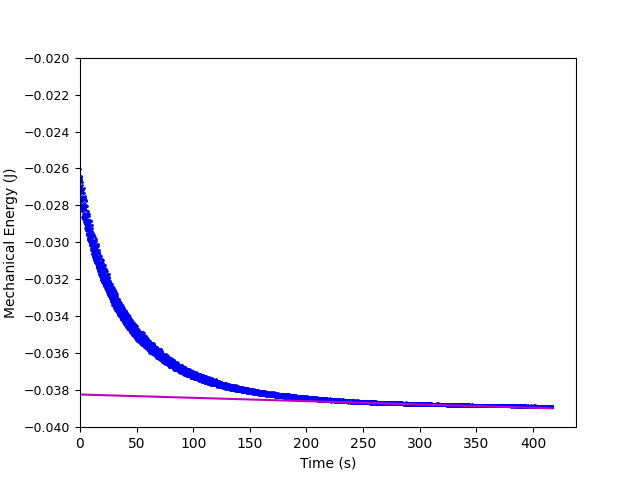
\includegraphics[width=0.5\linewidth]{mechanical-energy-linear-fit-300s}
                \caption{Mechanical energy over time with linear fit around $t=300$ seconds}
                \label{fig:mechanical-energy-linear-fit-300s}
            \end{figure}
            
            On this graph, even though this linear line of best fit is relatively accurate around $t=300$ seconds, it is not accurate for the rest of the graph, due to the fact that the rate of change of mechanical energy over time is not constant.
            However, unlike the previous graphs, this line of best fit is accurate for a longer period of time, since the rate of change of mechanical energy over time is more constant around $t=300$ seconds than it is around $t=100$ seconds.
            This is because as the mechanical energy falls, the maximum velocity of the mass decreases, which means there is less energy loss.\\
            \newline This is even more evident when we compare the rate of change of mechanical energy over time for all three of the linear fits that we calculated.
            
            
            The following graph shows the rate of change of mechanical energy over time for all three of the linear fits that we calculated:
            
            %figure mechanical-energy-linear-fit-all
            \begin{figure}[H]
                \centering
                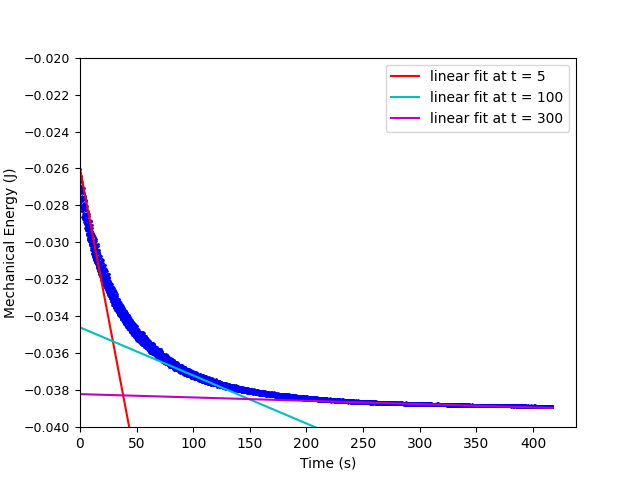
\includegraphics[width=0.5\linewidth]{mechanical-energy-linear-fit-all}
                \caption{Mechanical energy over time with linear fit around $t=100$ seconds}
                \label{fig:mechanical-energy-linear-fit-all}
            \end{figure}
            
            In this figure it is obvious that the rate of change of mechanical energy over time is not constant, and that it is decreasing over time.
            This is because as the mechanical energy falls, the maximum velocity of the mass decreases, which means there is less energy loss.
            The red line, which represents the rate of change of mechanical energy over time around $t=5$ seconds.
            This line has a significantly different slope than the cyan line, which represents the rate of change of mechanical energy over time around $t=100$ seconds.
            Furthermore, both of these lines have a significantly different slope than the green line, which represents the rate of change of mechanical energy over time around $t=300$ seconds.\\
            
            The prior process can be repeated for every point on the graph of mechanical energy over time, and a line of best fit can be calculated for each point. The following graph, for each point takes the mechanical energy of the point 2.8 seconds before and 2.8 seconds after, and graphs the rate of change of mechanical energy over time for that point.
            
            %figure mechanical-energy-rate-of-change
            \begin{figure}[H]
                \centering
                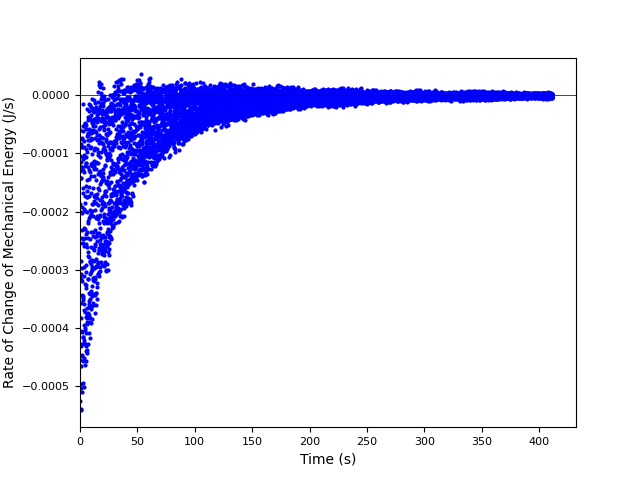
\includegraphics[width=0.5\linewidth]{mechanical-energy-rate-of-change}
                \caption{Mechanical energy over time, using a radius of 2.8 seconds}
                \label{fig:mechanical-energy-rate-of-change}
            \end{figure}
            
            The mechanical energy over time graph shows that the mechanical energy is always decreasing, and that the rate of change of mechanical energy over time is not constant.
            The change in mechanical energy near the end of the graph is significantly less than the change in mechanical energy near the beginning of the graph, most likely due to the fact that the velocity of the mass is decreasing, and thus the energy loss to air resistance is decreasing. %todo graph of velocity?
    
    
    \section{Discussion}
%    \subsection{Calculating the Average Rate of Change of Mechanical Energy Over Time}
        \subsection Question 1
            
            \subsubsection{Question 1a: Give the experimental average value for the rate of change of the mechanical energy of the oscillating mass with respect to time?}
                If we take the average of all of the rates of change of mechanical energy over time from figure~\ref{fig:mechanical-energy-rate-of-change}, we get that teh average rate of change of mechanical energy is $-0.000026 \frac{\text{ J}}{\text{ s}}$.
                %todo that number seems wrong
                This means that over the course of the experiment, the rate of change of mechanical energy was on average $-0.000026 \frac{\text{ J}}{\text{ s}}$.
            
            \subsubsection{Question 1b: What is your experimental rate of change of the mechanical energy of the oscillating mass with respect to time?}
                The rate of change of mechanical energy of the mass with respect to time depends based on the time. Based on figure~\ref{fig:mechanical-energy-rate-of-change} (reproduced below), the rate of change of mechanical energy of the mass with respect to time is $-0.000026 \frac{\text{ J}}{\text{ s}}$ at around $t=100$ seconds, $-0.0000018 \frac{\text{ J}}{\text{ s}}$ at around $t=300$ seconds, and $-0.000026 \frac{\text{ J}}{\text{ s}}$ at around $t=300$ seconds.
                
                %figure mechanical-energy-rate-of-change
                \begin{figure}[H]
                    \centering
                    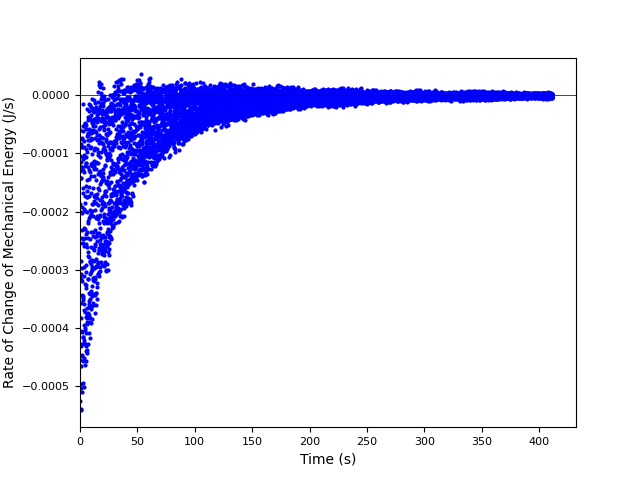
\includegraphics[width=0.5\linewidth]{mechanical-energy-rate-of-change}
                    \caption{Mechanical energy over time, using a radius of 2.8 seconds}
                    \label{fig:mechanical-energy-rate-of-change-2}
                \end{figure}

                $W_{\text{ext}} + W_{\text{int,nc}} = \Delta M$

        
        \subsection{Question 2: What are the energy transformations that are responsible for the change in mechanical energy?}
            The change in mechanical energy is caused primarily by air resistance, which is caused by the mass moving through the air.
            There are also some additional minor losses such as friction between the mass holder and the spring.
            
            The friction in both of these cases converts the mechanical energy of the mass into heat/thermal energy energy and the kinetic energy of the air.
            Specifically, it transfers the kinetic energy into heat/thermal energy, causing a decrease in the mechanical energy of the oscillating mass.
    
    
    \section{Potential Errors, Next Steps, and Future Improvements}
        \begin{itemize}
            \item Ultrasonic sensor's readings are not frequent enough
            \item The mass of the mass holder was not measured
            \item The spring is not massless
            \item The spring did not oscillate directly up and down
            \item The ultrasonic motion detector's velocity readings were unreliable
            \item The x0 position was not accurate
            \item Not enough data points were taken to find the spring constant.
            \item Multiple trials were not taken to find the change in mechanical energy over time.
            \item In the change in mechanical energy over time graph, there are points that show that the mechanical energy is sometimes increasing. However, there are no external or non-conservative forces that would cause the mechanical energy to increase. This is most likely due to the fact that the ultrasonic motion detector's velocity readings were unreliable, and the measurements of x0 and the mass were most likely unreliable as well. Having more runs and more reliable readings would help to fix this issue.
        \end{itemize}
    
    
    \section{Conclusion}
        In conclusion, the mechanical energy of the oscillating mass decreases over time, and the rate of change of mechanical energy over time is not constant.
        The mechanical energy of the oscillating mass decreases over time due to air resistance, which converts the mechanical energy of the mass into heat/thermal energy.
        The rate of change of mechanical energy over time is not constant because as the mechanical energy falls, the maximum velocity of the mass decreases, which means there is less energy loss.
        This is evident in the fact that the rate of change of mechanical energy over time is significantly less near the end of the experiment than it is near the beginning of the experiment.
        
        From this experiment we can conclude that the mechanical energy of an oscillating mass decreases over time, and that the rate of change of mechanical energy over time is not constant, and is primarily caused by air resistance.
        %todo update conclusion
        
        
        %todo add a graph with change in mech eng?
        %todo add appendix with all the data
        
        
%        \appendix
    
    
%    \section{Raw Oscillation Data}
%    The data has been processed so that the first peak occurs at 0 seconds.
%        \begin{table}
%            \centering
%            \caption{Raw Oscillation Data}
\begin{multicols}{2}
%    \scriptsize
%    \begin{table*}
%    \begin{tabular}{|c|c|c|c|}

\begin{longtable}{|c|c|c|c|}
%    \hline
%    Time [s] & Position [m] & Velocity [$\frac{\text{m}}{\text{s}}$] & Acceleration [$\frac{\text{m}}{\text{s}^2}$] \\
    \hline
    0.0      & 0.291        & -0.006                                 & -4.941                                       \\
    \hline
    0.05     & 0.281        & -0.289                                 & -4.01                                        \\
    \hline
    0.1      & 0.257        & -0.467                                 & -1.649                                       \\
    \hline
    0.15     & 0.227        & -0.478                                 & 1.285                                        \\
    \hline
    0.2      & 0.202        & -0.319                                 & 3.752                                        \\
    \hline
    0.25     & 0.191        & -0.046                                 & 4.882                                        \\
    \hline
    0.3      & 0.197        & 0.243                                  & 4.277                                        \\
    \hline
    0.35     & 0.218        & 0.447                                  & 2.132                                        \\
    \hline
    0.4      & 0.248        & 0.49                                   & -0.796                                       \\
    \hline
    0.45     & 0.275        & 0.354                                  & -3.42                                        \\
    \hline
    0.5      & 0.289        & 0.094                                  & -4.799                                       \\
    \hline
    0.55     & 0.286        & -0.198                                 & -4.467                                       \\
    \hline
    0.6      & 0.266        & -0.42                                  & -2.545                                       \\
    \hline
    0.65     & 0.237        & -0.491                                 & 0.285                                        \\
    \hline
    0.7      & 0.21         & -0.387                                 & 3.011                                        \\
    \hline
    0.75     & 0.193        & -0.144                                 & 4.66                                         \\
    \hline
    0.8      & 0.193        & 0.15                                   & 4.64                                         \\
    \hline
    0.85     & 0.21         & 0.39                                   & 2.961                                        \\
    \hline
    0.9      & 0.238        & 0.491                                  & 0.23                                         \\
    \hline
    0.95     & 0.267        & 0.417                                  & -2.596                                       \\
    \hline
    1.0      & 0.286        & 0.192                                  & -4.504                                       \\
    \hline
    1.05     & 0.289        & -0.103                                 & -4.78                                        \\
    \hline
    1.1      & 0.274        & -0.359                                 & -3.324                                       \\
    \hline
    1.15     & 0.247        & -0.485                                 & -0.687                                       \\
    \hline
    1.2      & 0.218        & -0.438                                 & 2.182                                        \\
    \hline
    1.25     & 0.197        & -0.234                                 & 4.265                                        \\
    \hline
    1.3      & 0.191        & 0.054                                  & 4.819                                        \\
    \hline
    1.35     & 0.203        & 0.321                                  & 3.646                                        \\
    \hline
    1.4      & 0.228        & 0.474                                  & 1.163                                        \\
    \hline
    1.45     & 0.258        & 0.455                                  & -1.735                                       \\
    \hline
    1.5      & 0.281        & 0.273                                  & -3.997                                       \\
    \hline
    1.55     & 0.289        & -0.005                                 & -4.826                                       \\
    \hline
    1.6      & 0.28         & -0.283                                 & -3.928                                       \\
    \hline
    1.65     & 0.257        & -0.459                                 & -1.61                                        \\
    \hline
    1.7      & 0.227        & -0.468                                 & 1.279                                        \\
    \hline
    1.75     & 0.203        & -0.31                                  & 3.693                                        \\
    \hline
    1.8      & 0.192        & -0.043                                 & 4.787                                        \\
    \hline
    1.85     & 0.198        & 0.241                                  & 4.17                                         \\
    \hline
    1.9      & 0.219        & 0.438                                  & 2.049                                        \\
    \hline
    1.95     & 0.248        & 0.478                                  & -0.81                                        \\
    \hline
    2.0      & 0.274        & 0.345                                  & -3.372                                       \\
    \hline
    2.05     & 0.288        & 0.088                                  & -4.71                                        \\
    \hline
    2.1      & 0.285        & -0.199                                 & -4.344                                       \\
    \hline
    2.15     & 0.265        & -0.412                                 & -2.434                                       \\
    \hline
    2.2      & 0.237        & -0.478                                 & 0.318                                        \\
    \hline
    2.25     & 0.21         & -0.375                                 & 2.964                                        \\
    \hline
    2.3      & 0.194        & -0.137                                 & 4.561                                        \\
    \hline
    2.35     & 0.194        & 0.15                                   & 4.519                                        \\
    \hline
    2.4      & 0.211        & 0.384                                  & 2.854                                        \\
    \hline
    2.45     & 0.239        & 0.48                                   & 0.157                                        \\
    \hline
    2.5      & 0.267        & 0.402                                  & -2.594                                       \\
    \hline
    2.55     & 0.285        & 0.18                                   & -4.403                                       \\
    \hline
    2.6      & 0.287        & -0.106                                 & -4.627                                       \\
    \hline
    2.65     & 0.273        & -0.353                                 & -3.187                                       \\
    \hline
    2.7      & 0.246        & -0.473                                 & -0.608                                       \\
    \hline
    2.75     & 0.218        & -0.422                                 & 2.169                                        \\
    \hline
    2.8      & 0.198        & -0.222                                 & 4.159                                        \\
    \hline
    2.85     & 0.193        & 0.056                                  & 4.676                                        \\
    \hline
    2.9      & 0.204        & 0.316                                  & 3.531                                        \\
    \hline
    2.95     & 0.229        & 0.463                                  & 1.116                                        \\
    \hline
    3.0      & 0.258        & 0.445                                  & -1.708                                       \\
    \hline
    3.05     & 0.28         & 0.267                                  & -3.931                                       \\
    \hline
    3.1      & 0.288        & -0.009                                 & -4.738                                       \\
    \hline
    3.15     & 0.279        & -0.28                                  & -3.828                                       \\
    \hline
    3.2      & 0.256        & -0.45                                  & -1.545                                       \\
    \hline
    3.25     & 0.227        & -0.458                                 & 1.282                                        \\
    \hline
    3.3      & 0.203        & -0.301                                 & 3.638                                        \\
    \hline
    3.35     & 0.193        & -0.038                                 & 4.68                                         \\
    \hline
    3.4      & 0.199        & 0.237                                  & 4.057                                        \\
    \hline
    3.45     & 0.22         & 0.429                                  & 1.99                                         \\
    \hline
    3.5      & 0.248        & 0.467                                  & -0.795                                       \\
    \hline
    3.55     & 0.274        & 0.338                                  & -3.299                                       \\
    \hline
    3.6      & 0.287        & 0.087                                  & -4.618                                       \\
    \hline
    3.65     & 0.284        & -0.195                                 & -4.278                                       \\
    \hline
    3.7      & 0.265        & -0.406                                 & -2.407                                       \\
    \hline
    3.75     & 0.237        & -0.472                                 & 0.325                                        \\
    \hline
    3.8      & 0.21         & -0.369                                 & 2.942                                        \\
    \hline
    3.85     & 0.194        & -0.133                                 & 4.508                                        \\
    \hline
    3.9      & 0.195        & 0.151                                  & 4.448                                        \\
    \hline
    3.95     & 0.212        & 0.38                                   & 2.782                                        \\
    \hline
    4.0      & 0.239        & 0.471                                  & 0.13                                         \\
    \hline
    4.05     & 0.266        & 0.394                                  & -2.558                                       \\
    \hline
    4.1      & 0.284        & 0.177                                  & -4.331                                       \\
    \hline
    4.15     & 0.287        & -0.105                                 & -4.548                                       \\
    \hline
    4.2      & 0.272        & -0.348                                 & -3.131                                       \\
    \hline
    4.25     & 0.246        & -0.465                                 & -0.604                                       \\
    \hline
    4.3      & 0.219        & -0.417                                 & 2.13                                         \\
    \hline
    4.35     & 0.198        & -0.22                                  & 4.108                                        \\
    \hline
    4.4      & 0.193        & 0.056                                  & 4.618                                        \\
    \hline
    4.45     & 0.205        & 0.312                                  & 3.475                                        \\
    \hline
    4.5      & 0.229        & 0.457                                  & 1.079                                        \\
    \hline
    4.55     & 0.258        & 0.437                                  & -1.713                                       \\
    \hline
    4.6      & 0.28         & 0.259                                  & -3.87                                        \\
    \hline
    4.65     & 0.287        & -0.01                                  & -4.626                                       \\
    \hline
    4.7      & 0.278        & -0.274                                 & -3.733                                       \\
    \hline
    4.75     & 0.256        & -0.439                                 & -1.515                                       \\
    \hline
    4.8      & 0.228        & -0.448                                 & 1.236                                        \\
    \hline
    4.85     & 0.204        & -0.297                                 & 3.542                                        \\
    \hline
    4.9      & 0.194        & -0.04                                  & 4.582                                        \\
    \hline
    4.95     & 0.2          & 0.231                                  & 3.989                                        \\
    \hline
    5.0      & 0.22         & 0.42                                   & 1.968                                        \\
    \hline
    5.05     & 0.248        & 0.458                                  & -0.758                                       \\
    \hline
    5.1      & 0.273        & 0.333                                  & -3.217                                       \\
    \hline
    5.15     & 0.286        & 0.087                                  & -4.53                                        \\
    \hline
    5.2      & 0.283        & -0.191                                 & -4.2                                         \\
    \hline
    5.25     & 0.264        & -0.397                                 & -2.357                                       \\
    \hline
    5.3      & 0.237        & -0.461                                 & 0.318                                        \\
    \hline
    5.35     & 0.211        & -0.36                                  & 2.871                                        \\
    \hline
    5.4      & 0.196        & -0.13                                  & 4.388                                        \\
    \hline
    5.45     & 0.196        & 0.145                                  & 4.341                                        \\
    \hline
    5.5      & 0.212        & 0.369                                  & 2.747                                        \\
    \hline
    5.55     & 0.239        & 0.462                                  & 0.161                                        \\
    \hline
    5.6      & 0.266        & 0.388                                  & -2.483                                       \\
    \hline
    5.65     & 0.283        & 0.176                                  & -4.24                                        \\
    \hline
    5.7      & 0.286        & -0.1                                   & -4.481                                       \\
    \hline
    5.75     & 0.272        & -0.342                                 & -3.092                                       \\
    \hline
    5.8      & 0.246        & -0.457                                 & -0.591                                       \\
    \hline
    5.85     & 0.219        & -0.408                                 & 2.098                                        \\
    \hline
    5.9      & 0.199        & -0.215                                 & 4.025                                        \\
    \hline
    5.95     & 0.194        & 0.055                                  & 4.512                                        \\
    \hline
    6.0      & 0.206        & 0.305                                  & 3.388                                        \\
    \hline
    6.05     & 0.23         & 0.445                                  & 1.055                                        \\
    \hline
    6.1      & 0.257        & 0.427                                  & -1.657                                       \\
    \hline
    6.15     & 0.279        & 0.254                                  & -3.775                                       \\
    \hline
    6.2      & 0.286        & -0.009                                 & -4.527                                       \\
    \hline
    6.25     & 0.278        & -0.267                                 & -3.661                                       \\
    \hline
    6.3      & 0.256        & -0.43                                  & -1.493                                       \\
    \hline
    6.35     & 0.228        & -0.44                                  & 1.218                                        \\
    \hline
    6.4      & 0.205        & -0.29                                  & 3.493                                        \\
    \hline
    6.45     & 0.195        & -0.036                                 & 4.502                                        \\
    \hline
    6.5      & 0.201        & 0.229                                  & 3.891                                        \\
    \hline
    6.55     & 0.221        & 0.412                                  & 1.886                                        \\
    \hline
    6.6      & 0.248        & 0.446                                  & -0.79                                        \\
    \hline
    6.65     & 0.273        & 0.32                                   & -3.174                                       \\
    \hline
    6.7      & 0.285        & 0.08                                   & -4.414                                       \\
    \hline
    6.75     & 0.282        & -0.189                                 & -4.068                                       \\
    \hline
    6.8      & 0.263        & -0.389                                 & -2.261                                       \\
    \hline
    6.85     & 0.237        & -0.448                                 & 0.336                                        \\
    \hline
    6.9      & 0.212        & -0.349                                 & 2.797                                        \\
    \hline
    6.95     & 0.197        & -0.127                                 & 4.276                                        \\
    \hline
    7.0      & 0.197        & 0.143                                  & 4.234                                        \\
    \hline
    7.05     & 0.213        & 0.362                                  & 2.669                                        \\
    \hline
    

%    \end{tabular}\label{tab:table}
%%        \end{table}
%\end{table*}
\end{longtable}
\end{multicols}


\end{document}
